\documentclass[twocolumn, amsmath, amsfonts, amssymb]{aastex62}
\usepackage{mathtools}
\usepackage{natbib}
\usepackage{bm}
\newcommand{\vdag}{(v)^\dagger}
\newcommand\aastex{AAS\TeX}
\newcommand\latex{La\TeX}


\newcommand{\Div}[1]{\ensuremath{\nabla\cdot\left( #1\right)}}
\newcommand{\DivU}{\ensuremath{\nabla\cdot\bm{u}}}
\newcommand{\angles}[1]{\ensuremath{\left\langle #1 \right\rangle}}
\newcommand{\KS}[1]{\ensuremath{\text{KS}(#1)}}
\newcommand{\KSstat}[1]{\ensuremath{\overline{\text{KS}(#1)}}}
\newcommand{\grad}{\ensuremath{\nabla}}
\newcommand{\RB}{Rayleigh-B\'{e}nard }
\newcommand{\stressT}{\ensuremath{\bm{\bar{\bar{\Pi}}}}}
\newcommand{\lilstressT}{\ensuremath{\bm{\bar{\bar{\sigma}}}}}
\newcommand{\nrho}{\ensuremath{n_{\rho}}}
\newcommand{\approptoinn}[2]{\mathrel{\vcenter{
	\offinterlineskip\halign{\hfil$##$\cr
	#1\propto\cr\noalign{\kern2pt}#1\sim\cr\noalign{\kern-2pt}}}}}

\newcommand{\appropto}{\mathpalette\approptoinn\relax}
\newcommand{\pro}{\ensuremath{\mathcal{P}_{\text{Ro}}\,}}


%% Tells LaTeX to search for image files in the 
%% current directory as well as in the figures/ folder.
\graphicspath{{./}{figs/}}


\received{\today}
\revised{\today}
\accepted{\today}
\submitjournal{ApJ}

\shorttitle{Predicting the Rossby number in convective experiments}
\shortauthors{Anders et al.}

\begin{document}
\defcitealias{anders&brown2017}{AB17}
\newcommand{\AB}{\citetalias{anders&brown2017}}

\title{Predicting the Rossby number in convective experiments}

\correspondingauthor{Evan H. Anders}
\email{evan.anders@colorado.edu}

\author{Evan H. Anders}
\affil{Dept. Astrophysical \& Planetary Sciences, University of Colorado -- Boulder, Boulder, CO 80309, USA}
\affil{Laboratory for Atmospheric and Space Physics, Boulder, CO 80303, USA}
\author{Cathryn M. Manduca}
\affil{Laboratory for Atmospheric and Space Physics, Boulder, CO 80303, USA}
\author{Benjamin P. Brown}
\affil{Dept. Astrophysical \& Planetary Sciences, University of Colorado -- Boulder, Boulder, CO 80309, USA}
\affil{Laboratory for Atmospheric and Space Physics, Boulder, CO 80303, USA}
\author{Jeffrey S. Oishi}
\affiliation{Department of Physics and Astronomy, Bates College, Lewiston, ME 04240, USA}
\author{Geoff Vasil}
\affiliation{University of Sydney School of Mathematics and Statistics, Sydney, NSW 2006, Australia}


\begin{abstract}
In this letter we study numerical simulations of stratified, compressible convection in a
rotational $f$-plane geometry. We define a new quantity, the Predictive Rossby number
(\pro), and show that it specifies the evolved Rossby number (Ro) of a convective simulation.
We examine the scaling of traditional fluid numbers and boundary layers along paths of constant
\pro.
\end{abstract}

\keywords{convection --- rotation --- turbulence}

%%%%% Body of the paper
\section{Introduction}
\label{sec:intro}
Convective flows in stars and planets are influenced by rotation. 
Rotating convection has been studied in great detail in
recent decades in both laboratory and numerical settings. The
properties of convection in the regime in which rotational forces are
insignificant are now well understood \citep{king&all2009, zhong&all2009, 
cheng&all2015}. Boussinesq convective theory is also robust
in the rapidly rotating regime \citep{julien&all2012, stellmach&all2014,
gastine&all2016}. We are not, however, aware of any well-developed
procedure for specifying the degree of rotational constraint
in a convective experiment \emph{a priori}. Rather, the rotational
constraint, measured by the evolved Rossby number
(Ro, the ratio of advective dynamics to rotational constraint), is a complex
combination of input parameters, such as convective driving and the
magnitude of the rotation vector.

A vast number of studies of rotating convection have been conducted in the astrophysical context.
Often these studies focus on questions inspired by the solar dynamo
\citep{glatzmaier&gilman1982, busse2002, brown&all2008,
brown&all2010, brown&all2011, augustson&all2012, guerrero&all2013, kapyla&all2014}.
Even when these simulations appear to be rotating at a rate similar to the Sun,
they can produce vastly different dynamics (such as anti-solar differential rotation).
These strange results may be the result of these systems having different evolved
values of the Rossby number than the Sun. Recent simulations and experiments are predicting
that the Rossby number of the deep interior of the Sun is low, and that this drastically
affects the behavior of the dynamics of the solar convection zone
\citep{featherstone&hindman2016, greer&all2016}.

In addition to it being very important to study the correct Rossby number
regime in solar convection studies, it also seems to be very important in
studies of planetary dynamos. For example, the balance between Lorentz forces
and rotational forces likely creates the observed differences between ice
giant and gas giant dynamos in our solar system \citep{soderlund&all2015}.
Furthermore, \cite{aurnou&king2017} suggest that many studies in planetary systems
have likely over-emphasized the importance of magnetism compared to rotation.

\begin{figure*}[t!]
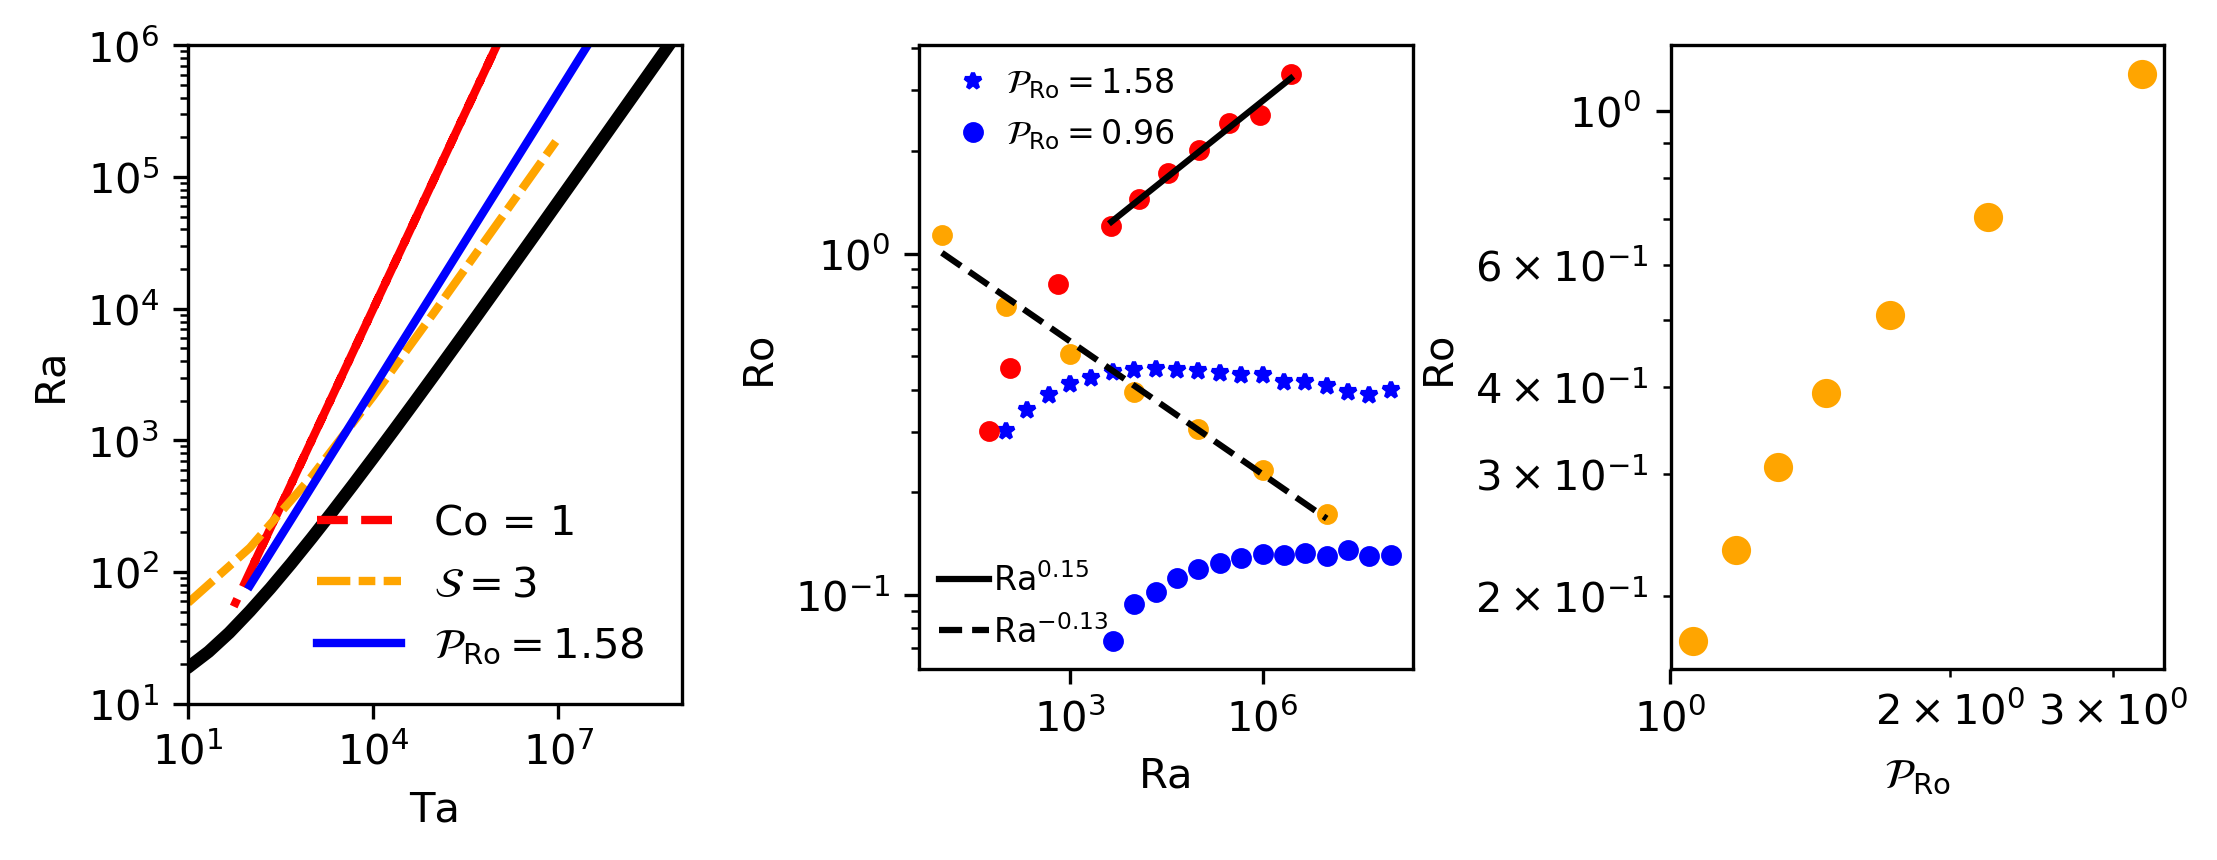
\includegraphics[width=\textwidth]{parameter_space.png}
\caption{(a) The critical Rayleigh number, as a function of the Taylor number, 
is plotted as a solid black line. Paths of constant Convective Rossby Number
(Co, green dashed line), constant supercriticality ($\mathcal{S}$, blue dash-dot line), and 
\pro (orange solid line) are shown through parameter space. (b) Evolved
Ro is plotted vs. Ra along multiple constant \pro
paths. For comparison, paths of constant $\mathcal{S}$ (blue squares; $\mathcal{S} = 3$ for
big squares and $\mathcal{S} = 2$ for small squares)
and constant Co (green triangles; Co = 1 for big triangles, Co = 0.3 for medium triangles,
and Co = 0.1 for small triangles) are shown.
Ro is roughly constant for a constant \pro, but changes drastically at constant Co and 
$\mathcal{S}$.
(c) The scaling of Ro with \pro is shown for $\mathcal{S} = (2,3)$.
At low Ro, both supercriticalities collapse onto a common scaling law of [NEED LAW].
At higher Ro, a different scaling law of [NEED LAW] is seen, and different supercriticalities
shift Ro.
\label{fig:parameter_space} }
\end{figure*}


It is clear that in studying astrophysical objects, the experimenter must 
study the proper Rossby number regime, and thus the proper degree of rotational
constraint.  In this work, our goal is to find a way of specifying the Rossby number
of convection in a simplified system through changing the input parameters.
In \cite{anders&brown2017} (hereafter \AB), we studied non-rotating, hydrodynamic, 
compressible convection in polytropic atmospheres. 
In this work, we extend the study of \AB$\,$ to rotationally-influenced, $f$-plane
atmospheres, as have been previously studied by e.g.,
\cite{brummell&all1996, brummell&all1998, calkins&all2015a}. Our goal is to determine
how the input parameters which we studied previously (which control the Mach number and
Reynolds number of the evolved flows) couple with a new input
parameter, the Taylor number (Ta, \cite{julien&all1996}), which sets the magnitude of the
rotational vector. 

In section  \ref{sec:experiment}, we describe our atmosphere, numerical
experiment, and paths through parameter space. In section \ref{sec:results}, we present
the results of our experiments and in section \ref{sec:discussion} we offer concluding remarks.

\section{Experiment} 
\label{sec:experiment}
We study fully compressible, stratified 
convection under precisely the same atmospheric model
as we previously did in \AB, and here
we have included rotation. We study polytropic atmospheres
with $n_\rho = 3$ density scale heights and a superadiabatic
excess of $\epsilon = 10^{-4}$ such that flows are at low Mach number.
As in previous work \citep{julien&all1996, brummell&all1996}, 
we study a domain in which the
gravity, $\bm{g} = -g\hat{z}$, and rotational vector, $\bm{\Omega} = \Omega \hat{z}$, 
are antiparallel.

We evolve the velocity ($\bm{u}$), temperature ($T$), 
and log density ($\ln\rho$) according to the
Fully Compressible Navier-Stokes equations in the same form presented in \AB, with the
addition of the Coriolis term, $2\bm{\Omega}\times\bm{u}$, to the left-hand side
of the momentum equation. We impose impenetrable, stress-free, fixed-temperature boundary
conditions at the top and bottom of the domain.

\begin{figure*}[t!]
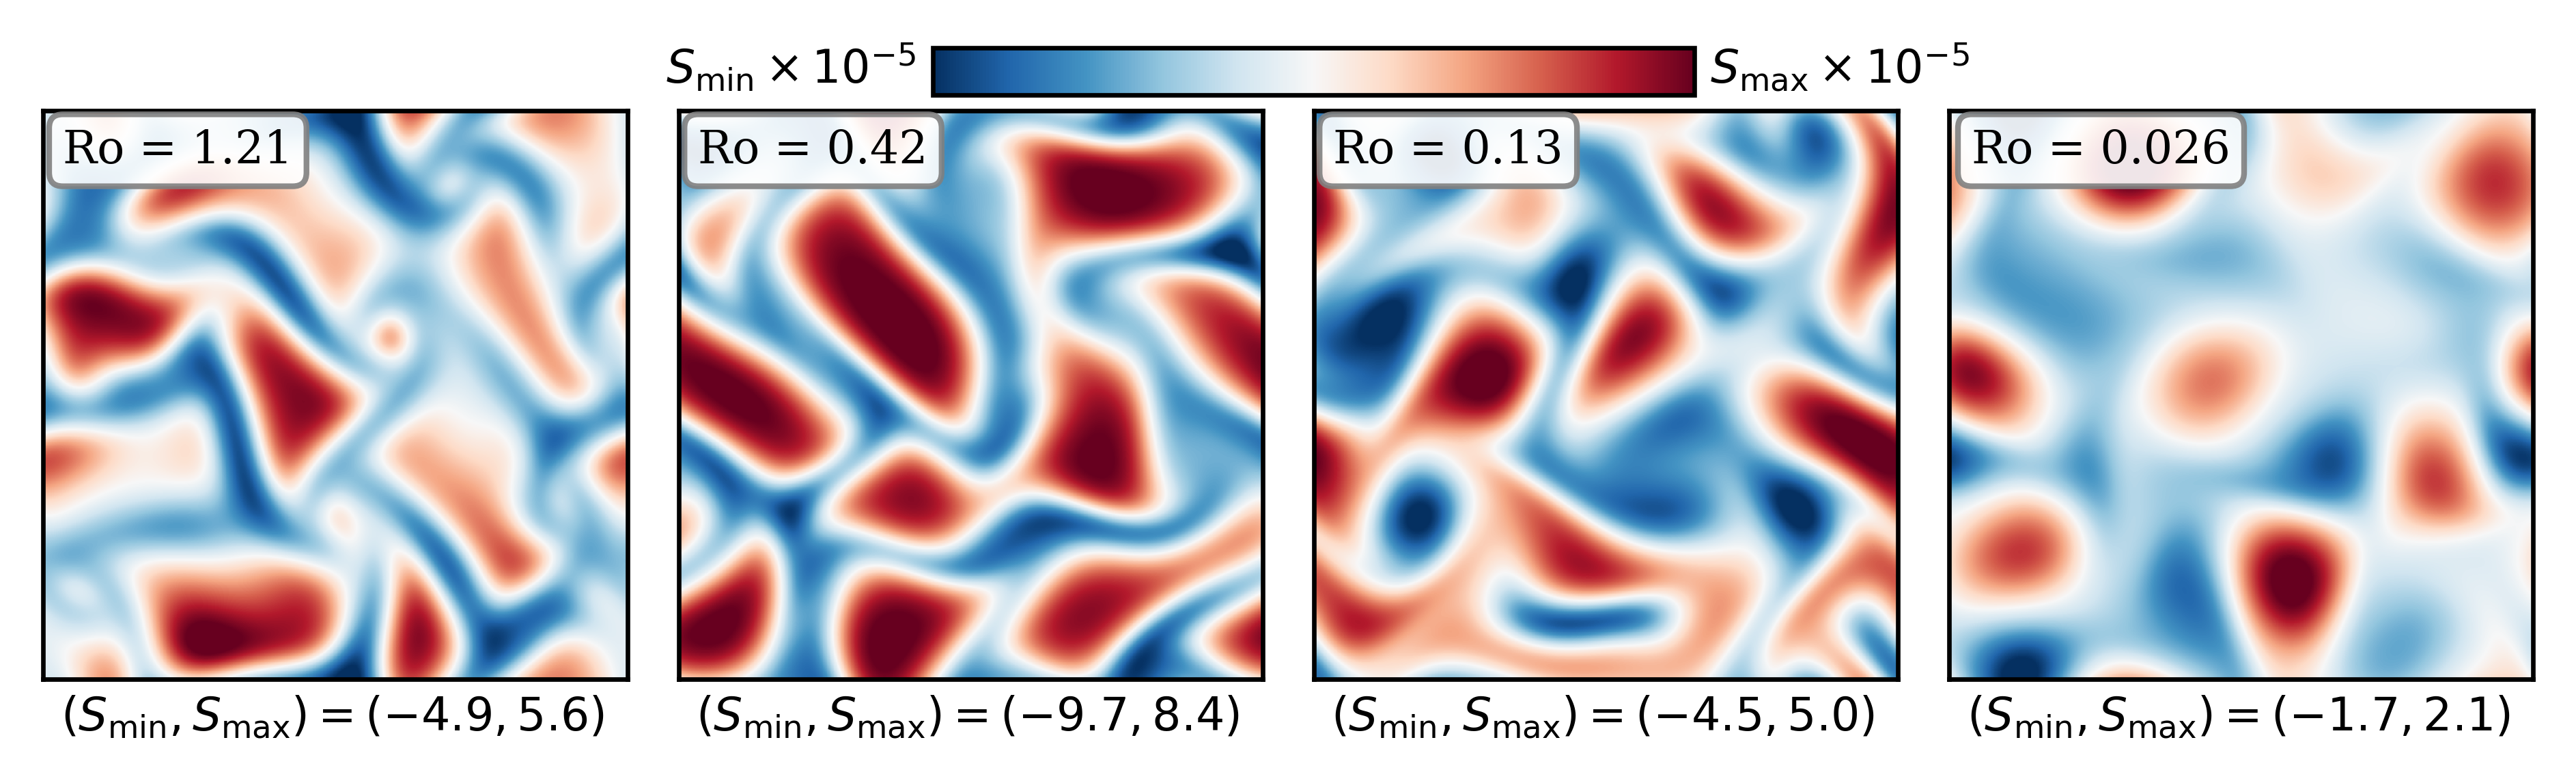
\includegraphics[width=\textwidth]{dynamics_plot.png}
\caption{ A horizontal slice of the evolved entropy field is plotted at $z = 0.95L_z$
for select simulations. The mean value of entropy at this height has been removed in all
cases. All runs displayed here have an evolved volume-averaged Re$\,\sim\,200$. 
As Ro decreases from O(1) on the left to O(0.1) on the right, and thus the rotational
constraint on the flow increases, significant changes in flow morphology are observed.
At Ro = 2.01, convective dynamics are not hugely dissimilar from the non-rotating
case where there are large upflows and narrow, fast downflow lanes (see e.g., \AB).
As the rotational constraint increases, the granular convective pattern gives way
to vortical columns, as seen at Ro = 0.13.
\label{fig:pretty_convection} }
\end{figure*}


The kinematic viscosity ($\nu$), thermal diffusivity ($\chi$), and strength of
rotation ($\Omega$) are set at the top of the domain by the Rayleigh number
(Ra), Prandtl number (Pr), and Taylor number (Ta),
\begin{equation}
\text{Ra} = \frac{g L_z^3 \Delta S / c_P}{\nu \chi}, \,\,\,
\text{Pr} = \frac{\nu}{\chi}, \,\,\,
\text{Ta} = \left(\frac{2 \Omega L_z^2}{\nu}\right)^2,
\end{equation}
where $L_z$ is the depth of the domain, 
$\Delta S = \epsilon n_\rho / m$ is the specific entropy difference between
$z = 0$ and $z = L_z$, and the specific heat at constant pressure is $c_P$.
Throughout this work we set Pr = 1.

As Ta increases, the wavenumber of convective onset, $k_{\text{crit}}$, also increases
\citep{calkins&all2015}. 
We study 3D cartesian convective domains with horizontal extents of
$x, y = [0, 4(2\pi/k_{\text{crit}})]$. 
We evolve our simulations using the Dedalus\footnote{\url{http://dedalus-project.org/}} 
pseudospectral framework, and our numerical methods are identical to those presented
in \AB.



As Ta increases, the critical value of Ra at which convection onsets,
Ra$_{\text{crit}}$, also increases (see the black line in Fig. \ref{fig:parameter_space}a). 
The linked nature of these crucial
control parameters makes it difficult to predict the rotational constraint of the evolved
fluid flows for a given set of input parameters. In this work, we will
explore three paths through Ra-Ta space:
\begin{equation}
\text{Ra} = 
\begin{cases}
\mathcal{S}\,\text{Ra}_\text{crit}(\text{Ta}), & (\text{I})\\
\text{Co}^2\text{Pr Ta}, & (\text{II}) \\
\pro^2 \text{Pr Ta}^{3/4} & (\text{III}).
\end{cases}
\label{eqn:paths}
\end{equation}
Paths on constraint I are at constant supercriticality, 
$\mathcal{S} \equiv \text{Ra}/\text{Ra}_{\text{crit}}$
(blue dash-dot line in Fig. \ref{fig:parameter_space}a).
Paths on constraint II are at a constant value of the classic
``Convective Rossby number'' (Co = Ra / [Pr Ta]), which has been used frequently 
in past work, and is intended to predict the rotational constraint of the
evolved solution (green dashed line in Fig. \ref{fig:parameter_space}a; 
\citet{julien&all1996, brummell&all1996}). Paths on constraint
III set constant a ratio which we call the ``Predictive Rossby Number,'' 
$\pro^2 = \text{Ra}/(\text{Pr}\text{Ta}^{3/4})$, 
(e.g., orange solid line in Fig. \ref{fig:parameter_space}a).
To our knowledge, these paths have not been
in the literature.

For each path defined in Eqn.~\ref{eqn:paths}, 
our goal is to study the magnitude of the rotational constraint
as quantified by the Rossby number,
\begin{equation}
\text{Ro} = \frac{|\grad\times \bm{u}|}{2 \Omega}.
\label{eqn:ro}
\end{equation}
If Ro remains constant over a large range of Ra along one of these paths,
then studies in which the magnitude of Ro is important should conduct
experiments along that path.



\section{Results \& Discussion}


\label{sec:results}
In Fig.~\ref{fig:parameter_space}a, the value of Ra$_{\text{crit}}$
is shown as a function of Ta, as
calculated by a linear instability analysis. A sample path for
each criterion in Eqn. \ref{eqn:paths} through
this parameter space is shown.
In Fig. \ref{fig:parameter_space}b, we display the scaling of Ro
with increasing Ra along various paths through parameter space.
We find that Ro increases on constant Co paths, decreases on constant $\mathcal{S}$
paths, and remains roughly constant along constant \pro$\,$ paths.
In Fig. \ref{fig:parameter_space}c, the behavior of Ro is shown as
a function of \pro$\,$ at constant $\mathcal{S}$.
At low Ro and \pro, in the rotationally constrained regime, the two parameters
are related according to the power law [INSERT HERE ONCE MORE DATA].
At higher Ro in the rotationally unconstrained regime, this scaling breaks down
to a [INSERT SCALING], with some offset at different values of $\mathcal{S}$.

\begin{figure}[t!]
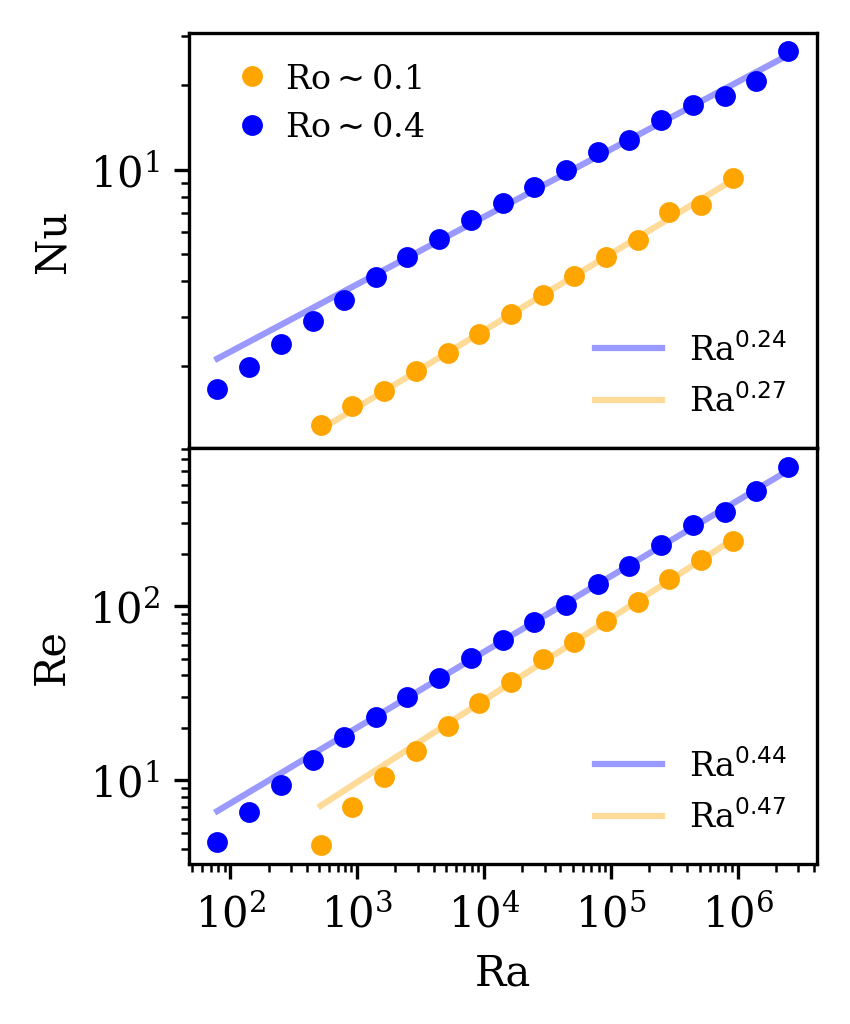
\includegraphics{./figs/nu_and_re.png}
\caption{Scaling laws for paths at $\pro = 1.58$ (Ro $\sim$ 0.4) and
$\pro = 0.96$ (Ro $\sim$ 0.1) are shown. 
(a) Evolved Nu vs. Ra. The scaling laws here are very reminiscent of classic \RB convection
theory \citep{ahlers&all2009}.
(b) Evolved Re vs. Ra.
The scaling seen here is nearly identical to scalings in nonrotating convection.
\label{fig:nu_and_re} }
\end{figure}

\begin{figure*}[ht!]
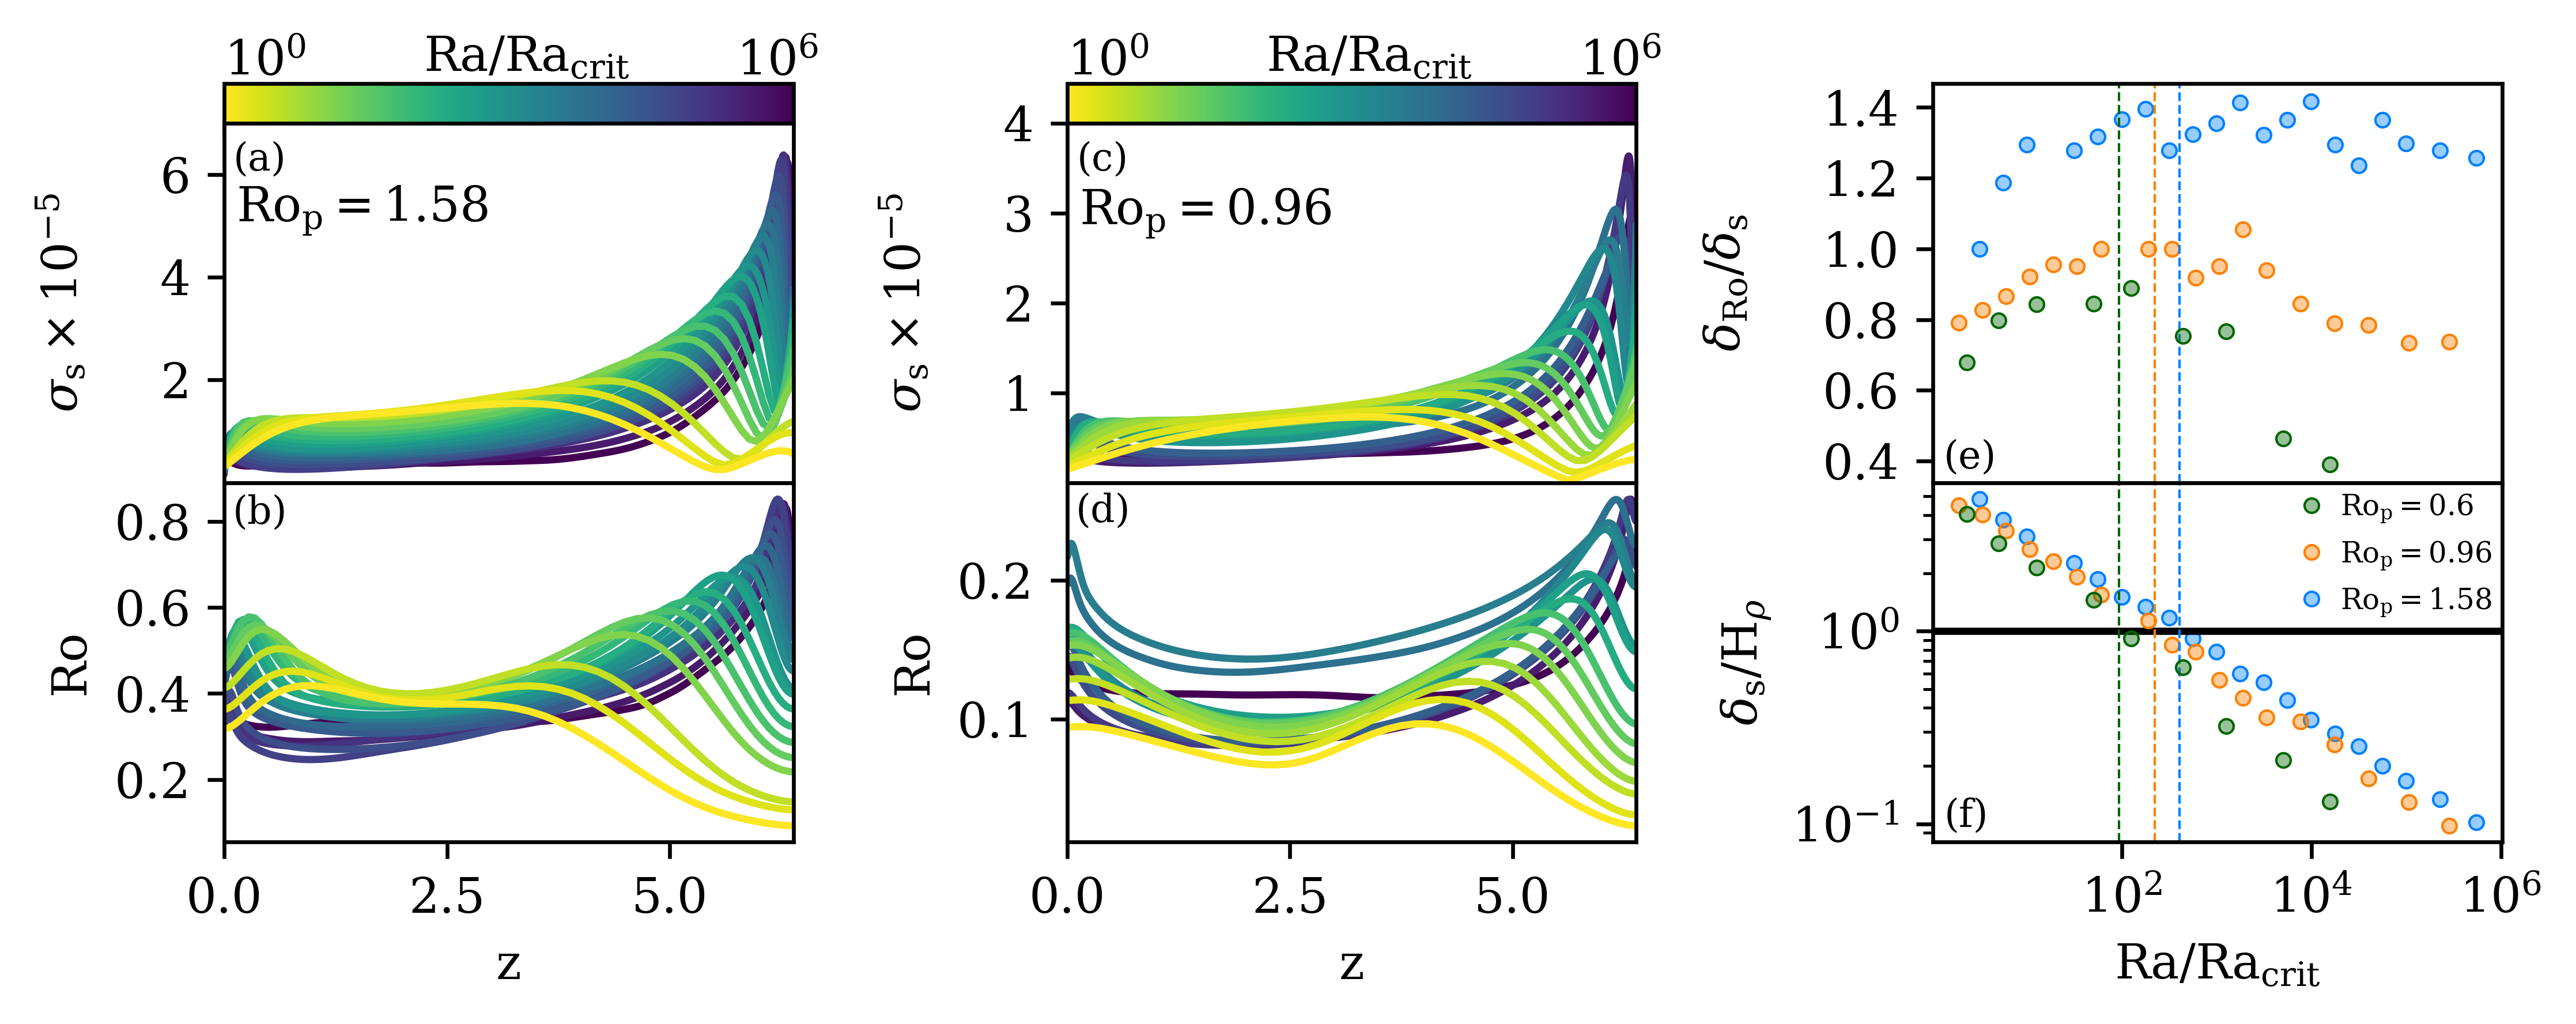
\includegraphics[width=\textwidth]{./figs/boundary_layers.png}
\caption{Horizontally-averaged profiles of the entropy gradient ($\grad s$, a)
and Rossby number (Ro, b) are shown vs. height for $\pro = 0.96$. 
Similar profiles are shown in (c) and (d) for $\pro = 1.58$. 
(c) The ratio of the sizes of the Ro boundary layer and $\grad s$ boundary layer are
shown. We find that for increasingly rotationally constrained flows, the Ro boundary layer
is increasingly thinner than the thermal boundary layer.
\label{fig:profiles_and_bls} }
\end{figure*}





In Fig.~\ref{fig:pretty_convection}, sample horizontal snapshots of the evolved entropy field
near the top of the domain are shown. 
In Fig.~\ref{fig:pretty_convection}a, a rotationally uncontrained flow at moderately high
Ro is shown. In Figs.~\ref{fig:pretty_convection}b\&c, increasingly rotationally constrained
convection is shown.
As Ro decreases, the
classic granular structure of convection (see e.g., Fig.~2 in \AB) gives way to vortical
columns of convection, as seen in rapidly rotating \RB convection \citep{stellmach&all2014}.
The select cases displayed in Fig.~\ref{fig:pretty_convection} have an evolved volume-averaged
Re$\,\sim\,$200.




We measure the Nusselt number (Nu, which quantifies heat transport in a convective
solution) as we did in \AB.
In Fig.~\ref{fig:nu_and_re}a, we show how Nu scales as a function
of Ra at fixed \pro. For constant \pro,
we find a scaling of $\text{Nu} \propto \text{Ra}^{0.27}$ in
the rotationally constrained regime. This is reminiscent of
classic scaling laws in non-rotating \RB convection \citep{ahlers&all2009}.
This suggests that changes in heat transport at constant \pro are driven by
changes in the boundary layer structure with increasing Ra.
In Fig. \ref{fig:nu_and_re}b, we plot the RMS Reynold's
number (Re $= |u| L_z / \nu$) as a function of Ra at fixed \pro, and find that 
$\text{Re} \propto \text{Ra}^{0.47} \sim \text{Ra}^{1/2}$ in the rotationally constrained regime,
which directly parallels the non-rotating regime in \AB.



In Fig. \ref{fig:profiles_and_bls}, we show time- and horizontally-averaged profiles of
Ro and the entropy gradient ($\grad s$). As Ra increases at a constant value of
\pro, both the entropy and rotational boundary layers become thinner. We measure the
thickness of the entropy boundary layer ($\delta_{\grad s}$) at the top of the domain by 
fitting a line within the boundary layer and finding when that line crosses zero. We measure
the thickness of the Ro boundary layer ($\delta_{\text{Ro}}$) 
as the height of the peak value of Ro within 
upper half of the domain.
In Fig. \ref{fig:profiles_and_bls}e, we plot $\delta_{\text{Ro}}/\delta_{\grad s}$, the ratio
of these two boundary layers. As anticipated, the dynamical boundary layer ($\delta_{\text{Ro}}$)
becomes relatively thinner with respect to the thermal boundary layer ($\delta_{\grad s}$)
as Ro decreases. [Need a sentence saying what this means]

\section{Discussion}
\label{sec:discussion}
In this letter, we studied low-Mach-number, stratified, compressible convection 
under the influence of rotation.
We examined three paths through Ra-Ta space, and showed that in the low-Ro, rotationally
constrained regime, the newly-defined 
Predictive Rossby number, $\pro = \text{Ra}/\text{Ta}^{3/4}$, determines the value of
the evolved Rossby number (Ro). While increasing Ra and holding \pro$\,$ constant,
we find scaling laws of heat transport (Nu) and turbulence (Re) that are nearly identical
to scaling laws seen in nonrotational convection.

Our results here suggest that experimenters can
can achieve whatever degree of rotational constraint they desire in their evolved solution
by choosing the proper value of \pro. Once that value is chosen, traditional experiments
in which the turbulent nature of the solutions is increased by increasing the Ra can be 
straightforwardly achieved. Preliminary results in 3D spherical convective systems suggest
that the results presented here are broadly applicable to rotational convection 
(Brown et al. 2019 in prep), even when the rotational vector is not every antiparallel to the
gravity vector.


\subsection{acknowledgements}
EHA acknowledges the support of NASA NESSF (insert fellowship number)
and the University of Colorado's George 
Ellery Hale Graduate Student Fellowship.
This work was additionally supported by  NASA LWS grant number NNX16AC92G.  
Computations were conducted 
with support by the NASA High End Computing (HEC) Program through the NASA 
Advanced Supercomputing (NAS) Division at Ames Research Center on Pleiades
with allocations GID s1647.

\newpage
\bibliography{biblio.bib}
\end{document}
